%%%%%%%%%%%%%%%%%%%%%%%%%%%%%%%%%%%%%%%%%
% Beamer Presentation
% LaTeX Template
% Version 1.0 (10/11/12)
%
% This template has been downloaded from:
% http://www.LaTeXTemplates.com
%
% License:
% CC BY-NC-SA 3.0 (http://creativecommons.org/licenses/by-nc-sa/3.0/)
%
%%%%%%%%%%%%%%%%%%%%%%%%%%%%%%%%%%%%%%%%%

%----------------------------------------------------------------------------------------
%	PACKAGES AND THEMES
%----------------------------------------------------------------------------------------

\documentclass{beamer}



\mode<presentation> {

% The Beamer class comes with a number of default slide themes
% which change the colors and layouts of slides. Below this is a list
% of all the themes, uncomment each in turn to see what they look like.

%\usetheme{default}
%\usetheme{AnnArbor}
%\usetheme{Antibes}
%\usetheme{Bergen}
%\usetheme{Berkeley}
%\usetheme{Berlin}
%\usetheme{Boadilla}
\usetheme{CambridgeUS}
%\usetheme{Copenhagen}
%\usetheme{Darmstadt}
%\usetheme{Dresden}
%\usetheme{Frankfurt}
%\usetheme{Goettingen}
%\usetheme{Hannover}
%\usetheme{Ilmenau}
%\usetheme{JuanLesPins}
%\usetheme{Luebeck}
%\usetheme{Madrid}
%\usetheme{Malmoe}
%\usetheme{Marburg}
%\usetheme{Montpellier}
%\usetheme{PaloAlto}
%\usetheme{Pittsburgh}
%\usetheme{Rochester}
%\usetheme{Singapore}
%\usetheme{Szeged}
%\usetheme{Warsaw}

% As well as themes, the Beamer class has a number of color themes
% for any slide theme. Uncomment each of these in turn to see how it
% changes the colors of your current slide theme.

%\usecolortheme{albatross}
%\usecolortheme{beaver}
%\usecolortheme{beetle}
%\usecolortheme{crane}
%\usecolortheme{dolphin}
%\usecolortheme{dove}
%\usecolortheme{fly}
%\usecolortheme{lily}
%\usecolortheme{orchid}
%\usecolortheme{rose}
\usecolortheme{seagull}
%\usecolortheme{seahorse}
%\usecolortheme{whale}
%\usecolortheme{wolverine}

%\setbeamertemplate{footline} % To remove the footer line in all slides uncomment this line
%\setbeamertemplate{footline}[page number] % To replace the footer line in all slides with a simple slide count uncomment this line

%\setbeamertemplate{navigation symbols}{} % To remove the navigation symbols from the bottom of all slides uncomment this line




%\usefonttheme[onlymath]{serif}
\usefonttheme{serif}
%\usefonttheme{professionalfonts}
%\usefonttheme{structuresmallcapsserif}
}

\usepackage{graphicx} % Allows including images
\usepackage{booktabs} % Allows the use of \toprule, \midrule and \bottomrule in tables
\usepackage[hangul]{kotex} % Korean support


%\graphicspath{ {D:/_PlayGround/Github/2016_thesis/tex/images/} } % image files path
\graphicspath{ {C:/My/Playground/Git/2016_Thesis/tex/images/} }

\setbeamertemplate{itemize items}[square]
%\setbeamertemplate{itemize items}[circle]
%\setbeamertemplate{itemize items}[ball]
%\setbeamertemplate{itemize items}[triangle]




%----------------------------------------------------------------------------------------
%	TITLE PAGE
%----------------------------------------------------------------------------------------

\title[]{빅데이터 분석을 위한 \\실시간 로지스틱 회귀모형에 관한 연구\\: 베이지안 접근법을 중심으로} % The short title appears at the bottom of every slide, the full title is only on the title page

\author{김동완} % Your name
\institute[고려대학교 정책대학원] % Your institution as it will appear on the bottom of every slide, may be shorthand to save space
{
고려대학교 정책대학원\\ % Your institution for the title page
데이터 통계학과\\
\medskip
\textit{} % Your email address
}
\date{\today} % Date, can be changed to a custom date


\begin{document}

\begin{frame}
\titlepage % Print the title page as the first slide
\end{frame}

\begin{frame}
\frametitle{Overview} % Table of contents slide, comment this block out to remove it
\tableofcontents % Throughout your presentation, if you choose to use \section{} and \subsection{} commands, these will automatically be printed on this slide as an overview of your presentation
\end{frame}



%----------------------------------------------------------------------------------------
%	PRESENTATION SLIDES
%----------------------------------------------------------------------------------------

%------------------------------------------------
\section{끓말} % Sections can be created in order to organize your presentation into discrete blocks, all sections and subsections are automatically printed in the table of contents as an overview of the talk
%------------------------------------------------

\subsection{개요} % A subsection can be created just before a set of slides with a common theme to further break down your presentation into chunks

\begin{frame}
\frametitle{새로운 형태의 데이터}

\begin{itemize}
\item 실제  IT 분야에서 해결해야하는 문제

    \begin{itemize}
    \setbeamertemplate{itemize items}[circle]
    \item TrueSkill과 같이 다량의 플레이어 게임 메칭 데이터를 이용해 플레이어의 승률을 계산하여 최적의 게임 메칭 상대를 찾는 문제
    \item 특정 Facebook 사용자의 timeline에 다양한 조건의 광고 중 어떤 광고를 노출 시켜야 광고 클릭 확률이 높을 것인지를 예측하는 문제
    \item 매출의 대부분을 차지하는 고부가 가치 유저(High-Valued Player)가 게임에서 이탈할 확률을 계산하는 문제
    \item 온라인 광고 퍼블리싱 상황에서 실시간으로 사이트마다 최적의 광고 선택 문제
    \end{itemize}

\item 이런 문제들의 특징
    \begin{itemize}
    \setbeamertemplate{itemize items}[circle]
    \item 유동적인 다 범주 변수
    \item 多  샘플, 실시간 분석
    \end{itemize}
\end{itemize}

\end{frame}
%------------------------------------------------





%----------------------------------------------------------------------------------------
%	PRESENTATION SLIDES
%----------------------------------------------------------------------------------------
\begin{frame}
\frametitle{새로운 형태의 데이터}

\begin{itemize}
\item 접근 방법
    \begin{itemize}
    \setbeamertemplate{itemize items}[circle]
    \item 유동적인 다 범주 변수\\
        $\rightarrow$ 해싱을 이용한 가변수 코딩(Feature Hashing)

    \item 多  샘플, 실시간 분석\\
        $\rightarrow$ 온라인 최적화
        \begin{itemize}
        \setbeamertemplate{itemize items}[triangle]
        \item 확률적 경사 하강법(SGD) vs 추정된 밀도 필터링(ADF)
        \end{itemize}

    \end{itemize}

\item 의문점
    \setbeamertemplate{itemize items}[circle]
    \begin{itemize}
    \item 기존의 배치 방식 대비 예측률
    \item 대용량 데이터에 대한 분석 속도
    \end{itemize}

\end{itemize}
\end{frame}
%------------------------------------------------





%----------------------------------------------------------------------------------------
%	PRESENTATION SLIDES
%----------------------------------------------------------------------------------------
%------------------------------------------------
\section{온라인 최적화 알고리즘과 해싱을 이용한 가변수 코딩} % Sections can be created in order to organize your presentation into discrete blocks, all sections and subsections are automatically printed in the table of contents as an overview of the talk
%------------------------------------------------

%----------------------------------------------------------------------------------------
%	PRESENTATION SLIDES
%----------------------------------------------------------------------------------------
\subsection{해싱을 이용한 가변수 코딩} % A subsection can be created just before a set of slides with a common theme to further break down your presentation into chunks

\begin{frame}
\frametitle{해싱을 이용한 가변수 코딩}
\begin{itemize}
    \item 해시 함수
    {\footnotesize
    \begin{itemize}
    \setbeamertemplate{itemize items}[circle]
    \item 해시 함수는 임의의 길이의 데이터를 고정된 길이의 데이터로 매핑하는 알고리즘.
    \item 암호화에 많이 사용됨
    \end{itemize}
    }

    \item 종류
    {\footnotesize
    \begin{itemize}
    \setbeamertemplate{itemize items}[circle]
    \item 암호화 해시
        \\: 복호화가 어려워야 함(MD5, SHA)
    \item 비암호화 해시
        \\: 분포적 특성과 속도가 중요(Murmur, City, Spooky)
        \\\quad $\rightarrow$ 데이터 분석에 사용
    \end{itemize}
    }
\end{itemize}
\end{frame}
%------------------------------------------------



%----------------------------------------------------------------------------------------
%	PRESENTATION SLIDES
%----------------------------------------------------------------------------------------
\begin{frame}
\frametitle{해싱을 이용한 가변수 코딩}
\begin{itemize}
    \item 해시 함수
    {\footnotesize
    \begin{itemize}
    \setbeamertemplate{itemize items}[circle]
    \item 해시 함수는 임의의 길이의 데이터를 고정된 길이의 데이터로 매핑하는 알고리즘.
    \item 암호화에 많이 사용됨
    \end{itemize}
    }

    \item 종류
    {\footnotesize
    \begin{itemize}
    \setbeamertemplate{itemize items}[circle]
    \item 암호화 해시
        \\: 복호화가 어려워야 함(MD5, SHA)
    \item 비암호화 해시
        \\: 분포적 특성과 속도가 중요(Murmur, City, Spooky)
        \\\quad $\rightarrow$ 데이터 분석에 사용
    \end{itemize}
    }
\end{itemize}
\end{frame}
%------------------------------------------------





%----------------------------------------------------------------------------------------
%	PRESENTATION SLIDES
%----------------------------------------------------------------------------------------
\begin{frame}
\frametitle{해싱을 이용한 가변수 코딩}
{\footnotesize
\begin{itemize}

    \item 데이터가 두개의 범주형 변수 $V_1 \in \{c_1,c_2,c_3\}$과 $V_2 \in \{c_4,c_5,c_6\}$로만 구성되어 있다고 할 때,

    \begin{itemize}
    \setbeamertemplate{itemize items}[circle]
    \item 일반적인 가변수 코딩
        \\: $n$건의 데이터에서 $i$번째 데이터 벡터 $[ x_{i1}, x_{i2} ]$는 \\~$[b_{11},b_{12},b_{21},b_{22}], b_{ij} \in \{0, 1\}$의 4자리 벡터로 가변수 코딩

    \item 해싱을 가변수 코딩
        \\: 데이터 값을 각각에 대한 해시 함수($H(\cdot)$)의 결과 값 벡터
         \\ ~$[ h_{i1} = H(x_{i1}), h_{i2} = H(x_{i2})], h_{ij} \in \mathbb{R}_{>0}$로 코딩
        \\: 해시 함수의 최대 비트 수를 b라 할때, $h_{ij}$의 최대값은 $2^b$이고,
        \\ ~ 실제로 필요한 예상되는 변수의 수가 $L$개로 제한된다면
        \\ ~~ $2^b ~mod~ L$을 $h_{ij}$ 대신 사용
    \end{itemize}


\end{itemize}
}
\end{frame}
%------------------------------------------------


%----------------------------------------------------------------------------------------
%	PRESENTATION SLIDES
%----------------------------------------------------------------------------------------
\begin{frame}
\frametitle{해싱을 이용한 가변수 코딩}

\begin{figure}
	\begin{center}
	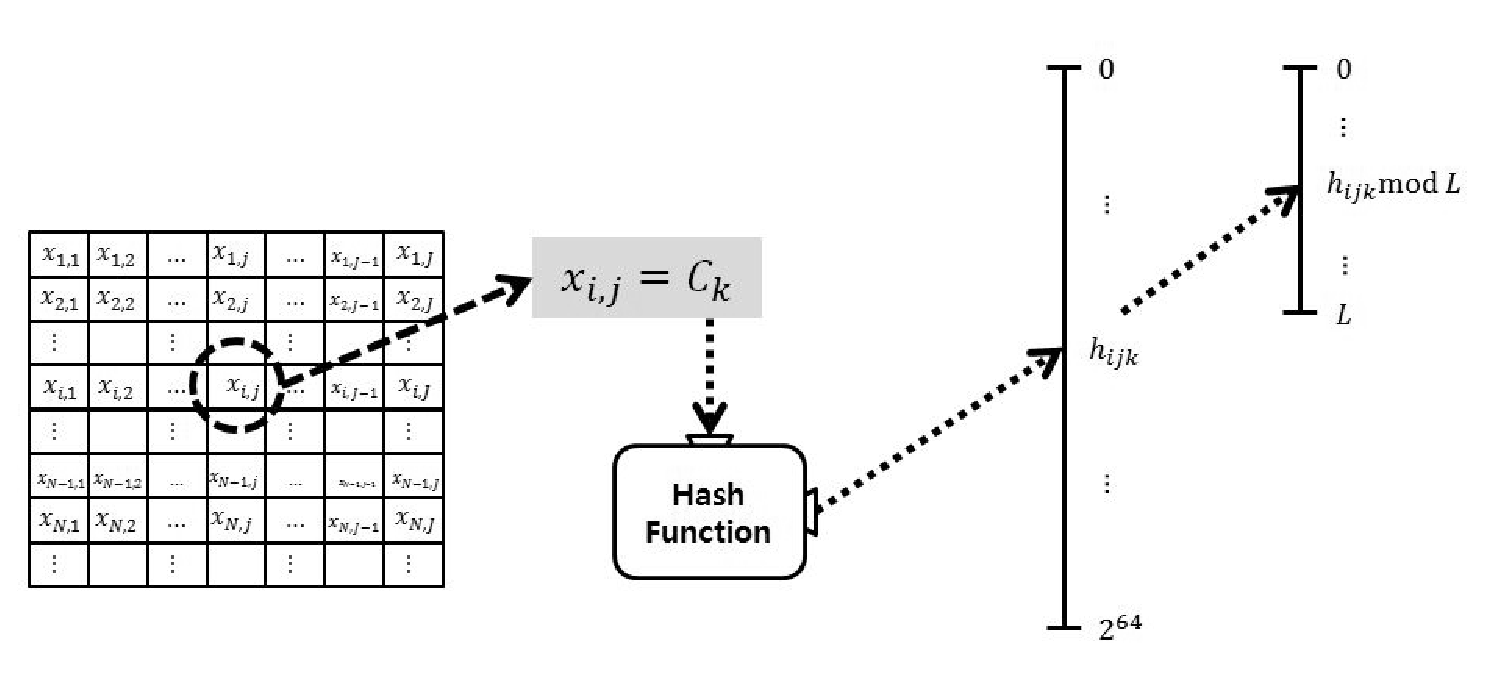
\includegraphics[scale=0.30]{hashing.eps} %730 * 430
    \end{center}
\end{figure}

{\footnotesize
\begin{itemize}

    \item 해싱을 이용한 가변수 코딩은 아래의 경우에도
        \\빈번한 가변수 코딩을 수행할 필요가 없어 효과적
    \\ \quad - 범주형 변수의 수와 각 범주를 구성하는 범주가 많을 경우
    \\ \quad - 범주의 수가 지속적으로 추가될 수 있는 경우
    \\ \quad - 실시간 분석이 요구되는 경우
\end{itemize}

}
\end{frame}
%------------------------------------------------





%----------------------------------------------------------------------------------------
%	PRESENTATION SLIDES
%----------------------------------------------------------------------------------------
\subsection{온라인 최적화 방법} % A subsection can be created just before a set of slides with a common theme to further break down your presentation into chunks

\begin{frame}
\frametitle{확률적 경사 하강법(Stochastic Gradient Descent)}
\begin{itemize}

\item {\scriptsize 최적화(optimization) 알고리즘의 하나인 경사하강법(Gradient descent)에서는 전체 샘플 데이터를 스캔 할 때마다 회귀 계수 추정치를 갱신}
\item {\scriptsize 비용함수(cost function)를 $J(w) = \frac{1}{2} \sum_{i}(target^{(i)} - output^{(i)})^{2}$ 라 할때 길이가 j인 계수 벡터(weight vector) $w_i$를 $w_{i+1}=w_{i}+\Delta w$로 갱신하는 매 반복에서 $j$개의 모수 추정치($w$)를 얼마만큼 줄일지 혹은 늘릴지 $\Delta w$ 값을 결정
\begin{eqnarray}
\Delta w_{j} 	&=& -\alpha \frac{\delta J}{\delta w_{j}} \\
							&=& -\alpha \sum_{i}(target^{(i)} - output^{(i)})(-x^{(i)_{j}}) \\
							&=& \alpha \sum_{i}(target^{(i)} - output^{(i)})(x^{(i)_{j}})
\end{eqnarray}
}

\item {\scriptsize 전체 샘플 데이터를 사용하는 대신 샘플 하나 혹은 일부분만을 사용하여 $w$ 값을 갱신해 가는 경사하강법을 확률적 경사 하강법이라 함}

\end{itemize}
\end{frame}

%------------------------------------------------





%----------------------------------------------------------------------------------------
%	PRESENTATION SLIDES
%----------------------------------------------------------------------------------------

\begin{frame}
\frametitle{추정된 밀도 필터링(Assumed-density filtering)}
\begin{itemize}

\item {\footnotesize ADF에서는 사후분포를 가우시안과 같은 특정 분포로 근사하는 방법으로서 예측-갱신-투영(predict-update-project)과정을 반복}
    \begin{itemize}
    \setbeamertemplate{itemize items}[circle]
    \item {\footnotesize 예측(predict)
        \\: 모수 $\theta$에 대한 $t-1$ 시점의 사전분포$q_{t-1}(\theta_{t-1})$와 \\
         ~~$t$시점의 관측치를 이용하여 \\
         ~~이후 시점 $t$에서의 $\theta$에 대한 사후예측분포, $q_{t|t-1}(\theta_{t})$를 구함}
    \item {\footnotesize 갱신(update)
        \\: 앞서 구한 사전분포와 사후예측분포를 이용하여
        \\~~$\theta$에 대한 사후분포, $\hat{p}(\theta_t)$를 구함}
    \item {\footnotesize 투영(project)
        \\: 마지막으로 이 사후 분포가 다루기 쉬운 형태가 아닌 경우가
        \\~~ 빈번하기 때문에 다루기 쉬운 분포로 투영(project)}
    \end{itemize}
\end{itemize}
\end{frame}

%------------------------------------------------






%----------------------------------------------------------------------------------------
%	PRESENTATION SLIDES
%----------------------------------------------------------------------------------------

\begin{frame}
\frametitle{추정된 밀도 필터링(Assumed-density filtering)}

{\footnotesize
    \begin{itemize}
    \item 근사 사전분포:
    $$q_{t-1}(\theta_{t-1}) \approx p(\theta_{t-1}|y_{1:t-1})$$
    \item 1단계 사후예측분포:
    $$q_{t|t-1}(\theta_t) = \int p(\theta_t | \theta_{t-1}) q_{t-1}(\theta_{t-1}) d\theta_{t-1}$$
    \item 사후분포:
    $$\hat{p}(\theta_t) = \frac{1}{Z_t}p(y_t | \theta_t)q_{t|t-1}(\theta_t)$$
    \item 정규화 상수(normalizing constant):
    $$Z_t = \int p(y_t | \theta_{t-1})q_{t|t-1}(\theta_{t})d\theta_{t}$$
    \item 근사 사후분포:
    $$q(\theta_t) = \arg\min_{q \in Q} \mathrm{KL}(\hat{p}(\theta_t || q(\theta_t)) $$
    \end{itemize}
}
\end{frame}

%------------------------------------------------






%----------------------------------------------------------------------------------------
%	PRESENTATION SLIDES
%----------------------------------------------------------------------------------------

\begin{frame}
\frametitle{추정된 밀도 필터링(Assumed-density filtering)}

{\footnotesize
    \begin{itemize}
    \item 일반화 선형 모형에서의 가우시안 근사
        \\ : 투영하려는 분포 $q$가 지수족 이므로 moment matching 대응 사용


    \begin{itemize}
    \setbeamertemplate{itemize items}[circle]
    {\scriptsize
        \item 일반화 선형 모형의 systematic component를 $s_t=\theta_t^T x_t$라 하면\\
        $s_t$의 사후 예측분포 $q_t(s_t)$는
        \begin{eqnarray}
        q_t(s_t) &\equiv& N(s_t; m_t, v_t)\nonumber
        \\ m_t &=& \int s_t \frac{1}{z_t} f(y_t|s_t) q_{t|t-1}(s_t)ds_t \nonumber
        \\ v_t &=& \int s^2_t \frac{1}{z_t} f(y_t|s_t) q_{t|t-1}(s_t) ds_t - m_t^2 \nonumber
        \\ z_t &=& \int f(y_t|s_t) q_{t|t-1}(s_t)ds_t \nonumber
        \\ f(y_t|s_t) &\equiv& Ber(y_t;\pi = sigmoid(s_t)) \nonumber
        \\ & =& \pi^{y_t} (1-\pi)^{(1-y_t)}, \quad y_t \in \{0,1\}
        \nonumber
        \end{eqnarray}

    }
    \end{itemize}
\end{itemize}
}
\end{frame}

%------------------------------------------------



%----------------------------------------------------------------------------------------
%	PRESENTATION SLIDES
%----------------------------------------------------------------------------------------

\begin{frame}
\frametitle{추정된 밀도 필터링(Assumed-density filtering)}

{\footnotesize
    \begin{itemize}
    \item 일반화 선형 모형에서의 가우시안 근사


    \begin{itemize}
    \setbeamertemplate{itemize items}[circle]
    {\scriptsize

        \item 가우스-에르미트 구적법을 사용하여 $s_t$의 사후분포를 근사하면,
        \begin{eqnarray}
        q_t(s_t) &=& N(s_t; \tilde{m}_t, \tilde{v}_t) \nonumber
        \\ \tilde{m}_t &=& \frac{1}{\tilde{z}_t} \sum_i \chi_i f(y_t; \chi_i ) \omega_i \nonumber
        \\ \tilde{v}_t &=& \frac{1}{\tilde{z}_t} \sum_i \chi^2_i f(y_t; \chi_i ) \omega_i - \tilde{m}^2_t \nonumber
        \\ \tilde{z}_t &=& \sum_i f(y_t; \chi_i ) \omega_i \nonumber
        \end{eqnarray}


        \item $q_{t|t-1}(s_{t-1})$을 $q_{t}(s_t)$로 갱신한 후 평균과 분산의 변화를 각각 $\sigma_m = m_t - m_{t|t-1}$과 $\sigma_v = v_t - v_{t|t-1}$라고 하면, $t$시점의 $i$번째 $\theta$의 분포는
            \begin{eqnarray}
               q(\theta_t,i) &\sim& N(\theta_{t,i};\mu_{t,i}, \sigma^2_{t,i})
            \end{eqnarray}
            $\mu_{t,i} = \mu_{t|t-1,i} + a_i \delta_m, \quad \sigma^2_{t,i} = \sigma^2_{t|t-1,i} + a^2_i \delta_v, \quad a_i \triangleq \frac{x_{t,i}\sigma^2_{t|t-1,i}}{\sum_j x^2_{t,j}\sigma^2_{t|t-1,i}}$

    }
    \end{itemize}
\end{itemize}
}
\end{frame}

%------------------------------------------------









%----------------------------------------------------------------------------------------
%	PRESENTATION SLIDES
%----------------------------------------------------------------------------------------

\section{사례연구} % Sections can be created in order to organize your presentation into discrete blocks, all sections and subsections are automatically printed in the table of contents as an overview of the talk
%------------------------------------------------

\subsection{타이타닉 탑승자 데이터} % A subsection can be created just before a set of slides with a common theme to further break down your presentation into chunks

\begin{frame}
\frametitle{소규모 데이터를 이용한 분석}


{\footnotesize
\begin{itemize}

    \item 타이타닉 탑승자들의 여러 특성에 따른 생존 여부를 나타내는 889건의 데이터를 800건의 훈련 데이터와 나머지 89건을 테스트 데이터로 나누고, 아래 3개 방법을 이용한 예측 성능을 비교
        \begin{itemize}
        \setbeamertemplate{itemize items}[circle]
        \item 최대우도 추정(MLE)
        \item 확률적 경사 하강법(SGD)
        \item 추정된 밀도 필터링(ADF)
        \end{itemize}
\end{itemize}
}

%\begin{table}[ht]

{\scriptsize
	\begin{center}%\centering
	\begin{tabular}{cccccccccc}
	\hline\hline
	%\toprule
	\textbf{} & \textbf{TP} & \textbf{FP} & \textbf{FN} & \textbf{TN} & \textbf{Accu} & \textbf{Prec} & \textbf{Recall} & \textbf{F1-Score} & \textbf{$logloss^1$}  \\
	\hline
	%\midrule
	
	\multicolumn {1}{l|}{MLE} & 24 & 9  & 5 & 41 & 0.843 & 0.727 & 0.826 & 0.774 & 0.423 \\ \hline
	\multicolumn {1}{l|}{SGD} & 22 & 11 & 6 & 50 & 0.809 & 0.667 & 0.786 & 0.721 & 0.411 \\ \hline
	\multicolumn {1}{l|}{ADF} & 21 & 12 & 7 & 49 & 0.787 & 0.636 & 0.750 & 0.688 & 0.437 \\ \hline

	\hline
	%\bottomrule
	\end{tabular}
    \end{center}
}



	\begin{flushright}
    {\tiny $1)~logloss = -\frac{1}{N}\sum_{i=1}^N {(y_i\log(p_i) + (1 - y_i)\log(1 - p_i))}$}
    \end{flushright}
%\end{table}

\end{frame}
%------------------------------------------------





%----------------------------------------------------------------------------------------
%	PRESENTATION SLIDES
%----------------------------------------------------------------------------------------


\subsection{온라인 광고 데이터} % A subsection can be created just before a set of slides with a common theme to further break down your presentation into chunks

\begin{frame}
\frametitle{대규모 데이터를 이용한 분석}


\begin{itemize}
\item 사례 분석을 위해 Criteo에서 데이터 분석 경연을 위해 공개한 4천 5백만건 상당의 온라인 광고 데이터 사용
    {\footnotesize
    \begin{itemize}
    \setbeamertemplate{itemize items}[circle]
    \item 데이터는 웹사이트 방문자가 해당 광고를 클릭 했으냐 혹은 하지 않았느냐를 나타내는 이항 반응변수와 광고의 특성을 나타내는 39개의 설명변수로 구성
    \item 각 설명변수는 범주형으로서 각 변수의 범주는 500개 이상이고 점차 새로운 범주가 등장
    \end{itemize}
    }
\end{itemize}

%sim 1
%1,000
{\scriptsize
	\begin{center}%\centering
	\begin{tabular}{ccccccc}
	\hline\hline %\toprule

    \multicolumn{5}{c}{\textbf{Training data size: $10^3$, Test data size: $10^3$}} & \textbf{} & \textbf{} \\

	\textbf{} & \textbf{Accu} & \textbf{Prec} & \textbf{Recall} & \textbf{F1-Score} & \textbf{$logloss^1$} & \textbf{exec time(sec)} \\

	\hline %\midrule
	
	\multicolumn {1}{l|}{SGD} & 0.716 & 0.380 & 0.526 & 0.441 & 0.570 & 0.308 \\ \hline
	\multicolumn {1}{l|}{ADF} & 0.702 & 0.343 & 0.437 & 0.384 & 0.570 & 0.461 \\ \hline

	\hline %\bottomrule
	\end{tabular}
    \end{center}
}


\end{frame}
%------------------------------------------------





%----------------------------------------------------------------------------------------
%	PRESENTATION SLIDES
%----------------------------------------------------------------------------------------

\begin{frame}
\frametitle{대규모 데이터를 이용한 분석}






%sim 3
%100,000
{\scriptsize
	\begin{center}%\centering
	\begin{tabular}{ccccccc}
	\hline\hline %\toprule

    \multicolumn{5}{c}{\textbf{Training data size: $10^5$, Test data size: $10^5$}} & \textbf{} & \textbf{} \\

	\textbf{} & \textbf{Accu} & \textbf{Prec} & \textbf{Recall} & \textbf{F1-Score} & \textbf{$logloss^1$} & \textbf{exec time(sec)} \\

	\hline %\midrule
	
	\multicolumn {1}{l|}{SGD} & 0.710 & 0.460 & 0.674 & 0.547 & 0.564 & 22.602 \\ \hline
	\multicolumn {1}{l|}{ADF} & 0.699 & 0.449 & 0.690 & 0.544 & 0.575 & 30.981 \\ \hline

	\hline %\bottomrule
	\end{tabular}
    \end{center}
}



% sim 5
%10,000,000
{\scriptsize
	\begin{center}%\centering
	\begin{tabular}{ccccccc}
	\hline\hline %\toprule

    \multicolumn{5}{c}{\textbf{Training data size: $10^7$, Test data size: $10^7$}} & \textbf{} & \textbf{} \\

	\textbf{} & \textbf{Accu} & \textbf{Prec} & \textbf{Recall} & \textbf{F1-Score} & \textbf{$logloss^1$} & \textbf{exec time(sec)} \\

	\hline %\midrule
	
	\multicolumn {1}{l|}{SGD} & 0.712 & 0.460 & 0.707 & 0.557 & 0.560 & 2148.999 \\ \hline
	\multicolumn {1}{l|}{ADF} & 0.713 & 0.461 & 0.709 & 0.558 & 0.559 & 2756.530 \\ \hline

	\hline %\bottomrule
	\end{tabular}
    \end{center}
}




{\footnotesize
\begin{itemize}
\setbeamertemplate{itemize items}[circle]
\item 데이터 크기가 작을 경우($10^3$) SGD가 다소 나은 예측 성능을 보임.
\item 데이터 크기가 커질수록 두 모형의 성능 차이는 줄어들고 ADF가 다소 나은 성능을 보임
\item 실행 속도는 3가지 데이터 크기($10^3$, $10^5$, $10^7$)에서 모두 SGD가 빠르나, 그 차이는 44\%, 37\%, 28\%로 데이터 크기가 커질수록 줄어듬.
\end{itemize}
}




\end{frame}
%------------------------------------------------



%----------------------------------------------------------------------------------------
%	PRESENTATION SLIDES
%----------------------------------------------------------------------------------------


\subsection{맺음말} % A subsection can be created just before a set of slides with a common theme to further break down your presentation into chunks

\begin{frame}
\frametitle{맺음말}

{\footnotesize
\begin{itemize}

\item 多 범주의 多 변수 데이터 분석에 있어서 해싱을 이용한 가변수 코딩의 유용성 확인
\item 온라인 방식의 적합 방법의 성능이 배치 방식에 비해 크게 떨어지지 않음.
\item 대규모 데이터에 대해서 '근사 방법을 이용한 베이지안 방법론'이 충분히 좋은 속도와 성능을 보임
\item 확률적 경사하강법에서는 모수별 step size의 초기값, 추정된 밀도 필터링에서는 모수별 초기 분산의 초기값에 예측 성능이 크게 영향을 받으나 데이터 크기가 커 질수록 그 영향은 줄어듬.
\item 변수 선택이나 변수간 교호작용 등 추후 고려해볼 것들이 있음.

\end{itemize}
}


\end{frame}
%------------------------------------------------












%------------------------------------------------

\begin{frame}
\Huge{\centerline{감사합니다.}}
\end{frame}

%----------------------------------------------------------------------------------------

%
% Reference
%


\end{document} 